%%%%
Las ecuaciones de Maxwell sin fuentes, considerando campos armónicos, se expresan como \cite{Balaniselectro} \cite{Fernandez}:
%%%%
\begin{align}
\divergencia{E} &= 0
\label{ec_apA:1}\\
\divergencia{H} &= 0
\label{ec_apA:2}\\
\rotor{E} &= -j\omega{\mu}\mathbf{H}
\label{ec_apA:3}\\
\rotor{H} &= j\omega{\varepsilon}\mathbf{E}
\label{ec_apA:4}
\end{align}
%%%%
En estas condiciones, las ecuaciónes de Maxwell conducen a las ecuaciónes de Helmholtz:
%%%%
\begin{subequations}
\label{grup_ec_apA:1}
\begin{align}
\laplaciano{E} + \gamma ^2\mathbf{E} &= 0
\label{ec_apA:5}\\
\laplaciano{H} + \gamma ^2\mathbf{H} &= 0
\label{ec_apA:6}
\end{align}
\end{subequations}
%%%%
donde:
%%%%
\begin{align}
&\gamma = \alpha + j\beta = \sqrt{j\omega\mu \left(\sigma + j\omega\varepsilon\right)}
\label{ec_apA:7}
\end{align}
%%%%
Suponiendo que dentro de la guía de onda no existen fuentes de campo:
%%%%
\begin{align}
\sigma = 0 \Longrightarrow\gamma^2 = -\omega^2\mu\varepsilon = -\left(\frac{2\pi}{\lambda}\right)^2 = - k^2
\label{ec_apA:8}
\end{align}
%%%%

%%%%
\section{Guías de onda rectangulares}
\label{sec_apendice_a_guia_rect}
%%%%

%%%%
Considerando la expresión del operador Laplaciano $\laplaciano{}$ en coordenadas cartesianas \cite{walfram_car_coord}, las ecuaciónes de Helmholtz \eqref{grup_ec_apA:1} quedan expresadas como:
%%%%
\begin{subequations}
\label{grup_ec_apA:2}
\begin{align}
\frac{\partial ^2\mathbf{E}}{\partial x^2} + \frac{\partial ^2\mathbf{E}}{\partial y^2} +  \frac{\partial ^2\mathbf{E}}{\partial z^2} + \gamma ^2\mathbf{E} &= 0
\label{ec_apA:9}\\
\frac{\partial ^2\mathbf{H}}{\partial x^2} + \frac{\partial ^2\mathbf{H}}{\partial y^2} +  \frac{\partial ^2\mathbf{H}}{\partial z^2} + \gamma ^2\mathbf{H} &= 0
\label{ec_apA:10}
\end{align}
\end{subequations}
%%%%
Por otro lado, a partir de las ecuaciónes de Maxwell del rotor para coordenadas cartesianas \cite{walfram_car_coord} se obtienen las expresiones:
%%%%
\begin{subequations}
\label{grup_ec_apA:3}
\begin{align}
\rotor{E} = -j\omega{\mu}\mathbf{H}\Longrightarrow
\begin{vmatrix}
\versor{x} & \versor{y} & \versor{z}\\
\dfrac{\partial}{\partial x} &\dfrac{\partial}{\partial y} &\dfrac{\partial}{\partial z}\\
E_x & E_y & E_z\\
\end{vmatrix}
&= - j\omega{\mu}\left(H_x\versor{x} + H_y\versor{y} + H_z\versor{z}\right)\Longrightarrow\notag\\
\frac{\partial E_z}{\partial y} - \frac{\partial E_y}{\partial z}  &= -j\omega{\mu}H_x
\label{ec_apA:11}\\
\frac{\partial E_x}{\partial z} - \frac{\partial E_z}{\partial x}  &= -j\omega{\mu}H_y
\label{ec_apA:12}\\
\frac{\partial E_y}{\partial x} - \frac{\partial E_x}{\partial y}  &= -j\omega{\mu}H_z
\label{ec_apA:13}\\
\rotor{H} = j\omega{\varepsilon}\mathbf{E}\Longrightarrow
\begin{vmatrix}
\versor{x} & \versor{y} & \versor{z}\\
\dfrac{\partial}{\partial x} &\dfrac{\partial}{\partial y} &\dfrac{\partial}{\partial z}\\
H_x & H_y & H_z\\
\end{vmatrix}
&= j\omega{\varepsilon}\left(E_x\versor{x} + E_y\versor{y} + E_z\versor{z}\right)\Longrightarrow\notag\\
\frac{\partial H_z}{\partial y} - \frac{\partial H_y}{\partial z}  &= j\omega{\varepsilon}E_x
\label{ec_apA:14}\\
\frac{\partial H_x}{\partial z} - \frac{\partial H_z}{\partial x}  &= j\omega{\varepsilon}E_y
\label{ec_apA:15}\\
\frac{\partial H_y}{\partial x} - \frac{\partial H_x}{\partial y}  &= j\omega{\varepsilon}E_z
\label{ec_apA:16}
\end{align}
\end{subequations}
%%%%
Las componentes transversales de los campos son solamente funciones de $x$ e $y$. Dado que los campos son armónicos y que se propagan a lo largo del eje \emph{z}, sus expresiones deben incorporar el factor $e^{j\omega t - \gamma_zz}$, pero no se incluye con el fin de facilitar la escritura.

Las expresiones resultantes de analizar las ecuaciónes de Maxwell del rotor \eqref{grup_ec_apA:3} son:
%%%%
\begin{subequations}
\label{grup_ec_apA:4}
\begin{align}
\frac{\partial E_z}{\partial y} + \gamma_z E_y &= - j\omega{\mu}H_x
\label{ec_apA:17}\\
- \gamma_z E_x - \frac{\partial E_z}{\partial x} &= - j\omega{\mu}H_y
\label{ec_apA:18}\\
\frac{\partial E_y}{\partial x} - \frac{\partial E_x}{\partial y} &= - j\omega{\mu}H_z
\label{ec_apA:19}\\
\frac{\partial H_z}{\partial y} + \gamma_z H_y &= j\omega{\varepsilon}E_x
\label{ec_apA:20}\\
- \gamma_z H_x - \frac{\partial H_z}{\partial x} &= j\omega{\varepsilon}E_y
\label{ec_apA:21}\\
\frac{\partial H_y}{\partial x} - \frac{\partial H_x}{\partial y} &= j\omega{\varepsilon}E_z
\label{ec_apA:22}
\end{align}
\end{subequations}
%%%%
y trabajando las expresiones \eqref{grup_ec_apA:4}, se obtienen las componentes de los campos:
%%%%
\begin{subequations}
\label{grup_ec_apA:5}
\begin{align}
E_x &= -\frac{1}{k^2_t}\left(\gamma_z\frac{\partial E_z}{\partial x} + j\omega\mu\frac{\partial H_z}{\partial y}\right)
\label{ec_apA:23}\\
E_y &= -\frac{1}{k^2_t}\left(\gamma_z\frac{\partial E_z}{\partial y} - j\omega\mu\frac{\partial H_z}{\partial x}\right)
\label{ec_apA:24}\\
H_x &= -\frac{1}{k^2_t}\left(\gamma_z\frac{\partial H_z}{\partial x} - j\omega\varepsilon\frac{\partial E_z}{\partial y}\right)
\label{ec_apA:25}\\
H_y &= -\frac{1}{k^2_t}\left(\gamma_z\frac{\partial H_z}{\partial y} + j\omega\varepsilon\frac{\partial E_z}{\partial x}\right)
\label{ec_apA:26}
\end{align}
\end{subequations}
%%%%
donde:
%%%%
\begin{align}
k^2_t = \gamma^2_z + k^2
\label{ec_apA:27}
\end{align}
%%%%
Las componentes longitudinales de los campos satisfacen las ecuaciones de Helmholtz:
%%%%
\begin{subequations}
\label{grup_ec_apA:6}
\begin{align}
\frac{\partial ^2E_z}{\partial x^2} + \frac{\partial ^2E_z}{\partial y^2} + k^2_tE_z &= 0
\label{ec_apA:28}\\
\frac{\partial ^2H_z}{\partial x^2} + \frac{\partial ^2H_z}{\partial y^2} + k^2_tH_z &= 0
\label{ec_apA:29}
\end{align}
\end{subequations}
%%%%
De todos los modos de propagación existentes, se considera el modo dominantes que es el TE$_{10}$. Para los modos TE se cumple que:
%%%%
\begin{align}
&E_z= 0 &H_z \not= 0
\label{ec_apA:30}
\end{align}
%%%%
por lo que las expresiones de las componentes de los campos \eqref{grup_ec_apA:5} se reducen a:
%%%%
\begin{subequations}
\label{grup_ec_apA:7}
\begin{align}
E_x &= - \frac{j\omega\mu}{k^2_t}\frac{\partial H_z}{\partial y}
\label{ec_apA:31}\\
E_y &= \frac{j\omega\mu}{k^2_t}\frac{\partial H_z}{\partial x}
\label{ec_apA:32}\\
H_x &= - \frac{\gamma_z}{k^2_t}\frac{\partial H_z}{\partial x}
\label{ec_apA:33}\\
H_y &= - \frac{\gamma_z}{k^2_t}\frac{\partial H_z}{\partial y}
\label{ec_apA:34}
\end{align}
\end{subequations}
%%%%
Sabiendo que $H_z\left(x,y\right) = H_z\left(x\right)H_z\left(y\right)$, es posible determinar el campo longitudinal $H_z$ aplicando separación de variables, por lo que la expresión \eqref{ec_apA:29} resulta:
%%%%
\begin{align}
&H_z\left(y\right)\frac{\partial^2H_z\left(x\right)}{\partial x^2} + H_z\left(x\right)\frac{\partial^2H_z\left(y\right)}{\partial y^2} + k_t^2H_z\left(x\right)H_z\left(y\right) = 0
\label{ec_apA:35}
\end{align}
%%%%
Dividiendo la expresión \eqref{ec_apA:35} por $H_z\left(x\right)H_z\left(y\right)$, se obtiene:
%%%%
\begin{align}
&\frac{1}{H_z\left(x\right)}\frac{\partial^2H_z\left(x\right)}{\partial x^2} + \frac{1}{H_z\left(y\right)}\frac{\partial^2H_z\left(y\right)}{\partial y^2} + k_t^2 = 0
\label{ec_apA:36}
\end{align}
%%%%
por lo que la ecuación de dos variables \eqref{ec_apA:29} ha quedado separada en dos ecuaciones de una variable, cuyas expresiones y soluciones son:
%%%%
\begin{subequations}
\label{grup_ec_apA:8}
\begin{align}
&\frac{\partial^2 H_z\left(x\right)}{\partial x^2} + k_x^2H_z\left(x\right) = 0\Longrightarrow H_z\left(x\right) = A\cos\left(k_xx\right) + B\sen\left(k_xx\right)
\label{ec_apA:37}\\
&\frac{\partial^2 H_z\left(y\right)}{\partial y^2} + k_y^2H_z\left(y\right) = 0\Longrightarrow H_z\left(y\right) = C\cos\left(k_yy\right) + D\sen\left(k_yy\right)
\label{ec_apA:38}
\end{align}
\end{subequations}
%%%%
donde:
%%%%
\begin{align}
k^2_t = k^2_x + k^2_y
\label{ec_apA:39}
\end{align}
%%%%
La componente longitudinal del campo $H_z$ puede expresarse como:
%%%%
\begin{align}
H_z\left(x,y\right) = H_z\left(x\right)H_z\left(y\right) = \left[A\cos\left(k_xx\right) + B\sen\left(k_xx\right)\right]\left[ C\cos\left(k_yy\right) + D\sen\left(k_yy\right)\right]
\label{ec_apA:40}
\end{align}
%%%%
por lo que las expresiones de sus derivadas parciales resultan:
%%%%
\begin{subequations}
\label{grup_ec_apA:9}
\begin{align}
\frac{\partial H_z}{\partial x} &= k_x\left[B\cos\left(k_xx\right) - A\sen\left(k_xx\right)\right]\left[C\cos\left(k_yy\right) + D\sen\left(k_yy\right)\right]
\label{ec_apA:41}\\
\frac{\partial H_z}{\partial y} &= k_y\left[A\cos\left(k_xx\right) + B\sen\left(k_xx\right)\right]\left[D\cos\left(k_yy\right) - C\sen\left(k_yy\right)\right]
\label{ec_apA:42}
\end{align}
\end{subequations}
%%%%
Considerando que el origen de coordenadas se ubica en el centro de la guía de onda rectangular, las condiciones de borde impuestas corresponden a las de la figura \ref{fig_apA:1}.
%%%%
\begin{figure} [H]
\centering 
\subfigure[Condiciones de borde reales.]{
\label{fig_apA:1}
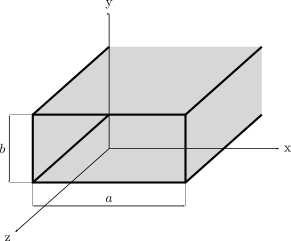
\includegraphics[scale = 1]{Figures/Apendice_A/apendiceA_1.pdf}}
\subfigure[Condiciones de borde auxiliares.]{
\label{fig_apA:2}
\includegraphics[scale = 1]{Figures/Apendice_A/apendiceA_2.pdf}}
\caption{Condiciones de borde para una guía de onda rectangular.}
\label{grup_fig_apA:1}
\end{figure}
%%%%
Para facilitar la resolución del problema, primero se determinan los campos para las condiciones de borde de la figura \ref{fig_apA:2} y luego se modifican las expresiones resultantes de los campos para que se correspondan a las condiciones de la figura \ref{fig_apA:1}.

Las componentes del campo eléctrico tangenciales a las paredes metálicas de la guía de onda se anulan, por lo que:
%%%%
\begin{subequations}
\label{grup_ec_apA:10}
\begin{align}
E_y\left(x=0\right) &= 0\Longrightarrow\frac{\partial H_z}{\partial x}\left(x=0\right) = 0
\label{ec_apA:43}\\
E_y\left(x=a\right) &= 0\Longrightarrow\frac{\partial H_z}{\partial x}\left(x=a\right) = 0
\label{ec_apA:44}\\
E_x\left(y=0\right) &= 0\Longrightarrow\frac{\partial H_z}{\partial y}\left(y=0\right) = 0
\label{ec_apA:45}\\
E_x\left(y=b\right) &= 0\Longrightarrow\frac{\partial H_z}{\partial y}\left(y=b\right) = 0
\label{ec_apA:46}
\end{align}
\end{subequations}
%%%%
Aplicando las condiciones de borde \eqref{grup_ec_apA:10}, se determina que:
%%%%
\begin{subequations}
\label{grup_ec_apA:11}
\begin{align}
B &= 0 &D &= 0
\label{ec_apA:47}\\
k_x &= \dfrac{m\pi}{a} &k_y &= \dfrac{n\pi}{b}
\label{ec_apA:48}
\end{align}
\end{subequations}
%%%%
por lo que las expresiones \eqref{grup_ec_apA:9} se reducen a:
%%%%
\begin{subequations}
\label{grup_ec_apA:12}
\begin{align}
&\frac{\partial H_z}{\partial x} = -AC\frac{m\pi}{a}\sen\left(\frac{m\pi}{a}x\right)\cos\left(\frac{n\pi}{b}y\right)
\label{ec_apA:49}\\
&\frac{\partial H_z}{\partial y} = -AC\frac{n\pi}{b}\cos\left(\frac{m\pi}{a}x\right)\sen\left(\frac{n\pi}{b}y\right)
\label{ec_apA:50}
\end{align}
\end{subequations}
%%%%
Las expresiones de los campos resultan:
%%%%
\begin{subequations}
\label{grup_ec_apA:13}
\begin{align}
E_x &= -j\frac{n\pi\omega\mu K}{b\gamma_t^2}\cos\left(\frac{m\pi}{a}x\right)\sen\left(\frac{n\pi}{b}y\right)
\label{ec_apA:51}\\
E_y &= j\frac{m\pi\omega\mu K}{a\gamma_t^2}\sen\left(\frac{m\pi}{a}x\right)\cos\left(\frac{n\pi}{b}y\right)
\label{ec_apA:52}\\
E_z &= 0
\label{ec_apA:53}\\
H_x &= -\frac{m\pi\gamma_zK}{a\gamma_t^2}\sen\left(\frac{m\pi}{a}x\right)\cos\left(\frac{n\pi}{b}y\right)
\label{ec_apA:54}\\
H_y &= -\frac{n\pi\gamma_zK}{b\gamma_t^2}\cos\left(\frac{m\pi}{a}x\right)\sen\left(\frac{n\pi}{b}y\right)
\label{ec_apA:55}\\
H_z &= -K\cos\left(\frac{m\pi}{a}x\right)\cos\left(\frac{n\pi}{b}y\right)
\label{ec_apA:56}
\end{align}
\end{subequations}
%%%%
donde $K = AC$ es una constante.

Luego de modificar las expresiones \eqref{grup_ec_apA:13} de acuerdo a las condiciones de borde de la figura \ref{fig_apA:2}, las componentes de los campos resultan:
%%%%
\begin{subequations}
\label{grup_ec_apA:14}
\begin{align}
&E_x = -j\frac{n\pi\omega\mu K}{b\gamma_t^2}\cos\left[\frac{m\pi}{a}\left(x + \frac{a}{2}\right)\right]\sen\left[\frac{n\pi}{b}\left(y + \frac{b}{2}\right)\right]
\label{ec_apA:57}\\
&E_y = j\frac{m\pi\omega\mu K}{a\gamma_t^2}\sen\left[\frac{m\pi}{a}\left(x + \frac{a}{2}\right)\right]\cos\left[\frac{n\pi}{b}\left(y + \frac{b}{2}\right)\right]
\label{ec_apA:58}\\
&E_z = 0
\label{ec_apA:59}\\
&H_x = -\frac{m\pi\gamma_zK}{a\gamma_t^2}\sen\left[\frac{m\pi}{a}\left(x + \frac{a}{2}\right)\right]\cos\left[\frac{n\pi}{b}\left(y + \frac{b}{2}\right)\right]
\label{ec_apA:60}\\
&H_y = -\frac{n\pi\gamma_zK}{b\gamma_t^2}\cos\left[\frac{m\pi}{a}\left(x + \frac{a}{2}\right)\right]\sen\left[\frac{n\pi}{b}\left(y + \frac{b}{2}\right)\right]
\label{ec_apA:61}\\
&H_z = -K\cos\left[\frac{m\pi}{a}\left(x + \frac{a}{2}\right)\right]\cos\left[\frac{n\pi}{b}\left(y + \frac{b}{2}\right)\right]
\label{ec_apA:62}
\end{align}
\end{subequations}
%%%%
donde la combinación de los índices $m$ y $n$ define un modo de propagación TE posible, que se designa como modo TE$_{\text{mn}}$.

Para cada modo en particular, es necesario que $\gamma_z$ sea imaginario para que exista propagación, ya que en caso contrario el factor de propagación se convierte en factor de atenuación. A partir de las expresiones \eqref{ec_apA:27}, \eqref{ec_apA:39} y \eqref{ec_apA:48}, $\gamma_z$ queda expresado como:
%%%%
\begin{align}
&\gamma_z = \sqrt{k^2_x + k^2_y - k^2} = \sqrt{\left(\frac{m\pi}{a}\right)^2 + \left(\frac{n\pi}{b}\right)^2 - \left(\frac{2\pi f}{v}\right)^2}
\label{ec_apA:63}
\end{align}
%%%%
La frecuencia a la cual $\gamma_z = 0$ se denomina \emph{frecuencia de corte}, cuya expresión es:
%%%%
\begin{align}
&f_c = \frac{v}{2\pi}\sqrt{\left(\frac{m\pi}{a}\right)^2 + \left(\frac{n\pi}{b}\right)^2}
\label{ec_apA:64}
\end{align}
%%%%
Combinando las expresiones \eqref{ec_apA:63} y \eqref{ec_apA:64} se determina el factor de fase $\beta$, cuya expresión es:
%%%%
\begin{align}
&\beta = k\sqrt{1 - \left(\dfrac{f_c}{f}\right)^2}
\label{ec_apA:65}
\end{align}
%%%%
Empleando la expresión \eqref{ec_apA:65} se determina la longitud de onda en la guía de onda $\lambda_g$, que queda expresada como:
%%%%
\begin{align}
&\lambda_g = \dfrac{2\pi}{\beta} = \dfrac{\lambda_0}{\sqrt{1 - \left(\dfrac{f_c}{f}\right)^2}}
\label{ec_apA:66}
\end{align}
%%%%
La impedancia de onda para los modos de propagación TE se expresa como:
%%%%
\begin{align}
&\eta_{TE} = \dfrac{E_x}{H_y} = -\dfrac{E_y}{H_x} = \dfrac{\eta}{\sqrt{1 - \left(\dfrac{f_c}{f}\right)^2}}
\label{ec_apA:67}
\end{align}
%%%%
Para el modo de propagación TE$_{10}$, las expresiones de las componentes de los campos resultan:
%%%%
\begin{subequations}
\label{grup_ec_apA:15}
\begin{align}
E_x &= 0
\label{ec_apA:68}\\
E_y &= j\frac{\pi\omega\mu K}{a\gamma_t^2}\cos\left(\frac{\pi}{a}x\right)
\label{ec_apA:69}\\
E_z &= 0
\label{ec_apA:70}\\
H_x &= -\frac{\pi\gamma_zK}{a\gamma_t^2}\cos\left(\frac{\pi}{a}x\right)
\label{ec_apA:71}\\
H_y &= 0
\label{ec_apA:72}\\
H_z &= K\sen\left(\frac{\pi}{a}x\right)
\label{ec_apA:73}
\end{align}
\end{subequations}
%%%%
y la frecuencia de corte:
%%%%
\begin{align}
&f_c = \frac{v}{2a}
\label{ec_apA:74}
\end{align}
%%%%
En la sección \ref{sec_fundamentos_principio} se dedujo que solamente las componenetes tangenciales de los campos sobre una abertura son las responsables de la radiación. Si se considera una guía de onda rectangular con un extremo abierto, será el extremo abierto de la guía el que cumplirá la función de abertura. A los fines de resolver el problema de radiación, puede considerarse que los campos sobre la abertura son las componentes transversales de los campos en la guía de onda, por lo que:
%%%%
\begin{subequations}
\label{grup_ec_apA:16}
\begin{align}
\mathbf{E}_a &= j\frac{\pi\omega\mu K}{a\gamma_t^2}\cos\left(\frac{\pi}{a}x\right)\versor{y}
\label{ec_apA:75}\\
\mathbf{H}_a &= -\frac{\pi\gamma_zK}{a\gamma_t^2}\cos\left(\frac{\pi}{a}x\right)\versor{x}
\label{ec_apA:76}
\end{align}
\end{subequations}
%%%%
Si las dimensiones de la abertura son grandes comparadas a la longitud de onda, los campos sobre la abertura $\mathbf{E}_a$ y $\mathbf{H}_a$ están relacionados entre sí a través de la expresión:
%%%%
\begin{align}
&\mathbf{H}_a = \versor{n}\prodvec\frac{\mathbf{E}_a}{\eta_{TE}} \simeq \versor{n}\prodvec\frac{\mathbf{E}_a}{\eta}
\label{ec_apA:77}
\end{align}
%%%%
y tomando que:
%%%%
\begin{align}
&E_0 = j\frac{\pi\omega\mu K}{a\gamma_t^2}
\label{ec_apA:78}
\end{align}
%%%%
las expresiones \eqref{grup_ec_apA:16} se reducen a:
%%%%
\begin{subequations}
\label{grup_ec_apA:17}
\begin{align}
\mathbf{E}_a &= E_y\,\versor{y} = E_0\cos\left(\frac{\pi}{a}x\right)\versor{y}
\label{ec_apA:79}\\
\mathbf{H}_a &= -\frac{E_y}{\eta}\,\versor{x} = - \frac{E_0}{\eta}\cos\left(\frac{\pi}{a}x\right)\versor{x}
\label{ec_apA:80}
\end{align}
\end{subequations}
%%%%

%%%%
\section{Guías de onda cilíndricas}
\label{sec_apendice_a_guia_cili}
%%%%

%%%%
Considerando la expresión del operador Laplaciano $\laplaciano{}$ en coordenadas cilíndricas \cite{walfram_sphe_coord}, las ecuaciónes de Helmholtz \eqref{grup_ec_apA:1} quedan expresadas como:
%%%%
\begin{subequations}
\label{grup_ec_apA:18}
\begin{align}
\frac{1}{\rho}\frac{1}{\partial\rho}\left(\!\rho\,\frac{\partial\mathbf{E}}{\partial\rho}\right) + \frac{1}{\rho^2}\frac{\partial ^2\mathbf{E}}{\partial\phi^2} +  \frac{\partial ^2\mathbf{E}}{\partial z^2} + \gamma ^2\mathbf{E} &= 0
\label{ec_apA:81}\\
\frac{1}{\rho}\frac{1}{\partial\rho}\left(\!\rho\,\frac{\partial\mathbf{H}}{\partial\rho}\right) + \frac{1}{\rho^2}\frac{\partial ^2\mathbf{H}}{\partial\phi^2} +  \frac{\partial ^2\mathbf{H}}{\partial z^2} + \gamma ^2\mathbf{H} &= 0
\label{ec_apA:82}
\end{align}
\end{subequations}
%%%%
Por otro lado, a partir de las ecuaciónes de Maxwell del rotor para coordenadas cilíndricas \cite{walfram_sphe_coord} se obtienen las expresiones:
%%%%
\begin{subequations}
\label{grup_ec_apA:19}
\begin{align}
\rotor{E} = -j\omega\mu\mathbf{H}\Longrightarrow\frac{1}{\rho}
\begin{vmatrix}
\versor{\uprho} & \rho\versor{\upphi} & \versor{z} \\
\dfrac{\partial}{\partial\rho} &\dfrac{\partial}{\partial\phi} &\dfrac{\partial}{\partial z} \\
E_{\rho} & \rho E_{\phi} & E_z \\
\end{vmatrix}
&= -j\omega\mu\left(H_{\rho}\versor{\uprho} + H_{\phi}\versor{\upphi} + H_z\versor{z}\right)\Longrightarrow\notag\\
\frac{1}{\rho}\frac{\partial E_z}{\partial\phi} - \frac{\partial E_{\phi}}{\partial z}  &= -j\omega\mu H_{\rho}
\label{ec_apA:83}\\
\frac{\partial E_{\rho}}{\partial z} - \frac{\partial E_z}{\partial\rho} & = -j\omega\mu H_{\phi}
\label{ec_apA:84}\\
\frac{1}{\rho}\left(\frac{\partial\left(\rho E_{\phi}\right)}{\partial\rho} - \frac{\partial E_{\rho}}{\partial\phi}\right)  &= -j\omega\mu H_z
\label{ec_apA:85}\\
\rotor{H} = j\omega\varepsilon\mathbf{E}\Longrightarrow\frac{1}{\rho}
\begin{vmatrix}
\versor{\uprho} & \rho\versor{\upphi} & \versor{z} \\
\dfrac{\partial}{\partial\rho} &\dfrac{\partial}{\partial\phi} &\dfrac{\partial}{\partial z} \\
H_{\rho} & \rho H_{\phi} & H_z \\
\end{vmatrix}
&= j\omega\varepsilon\left(E_{\rho}\versor{\uprho} + E_{\phi}\versor{\upphi} + E_z\versor{z}\right)\Longrightarrow\notag\\
\frac{1}{\rho}\frac{\partial H_z}{\partial\phi} - \frac{\partial H_{\phi}}{\partial z}  &= j\omega\varepsilon E_{\rho}
\label{ec_apA:86}\\
\frac{\partial H_{\rho}}{\partial z} - \frac{\partial H_z}{\partial\rho} & = j\omega\varepsilon E_{\phi}
\label{ec_apA:87}\\
\frac{1}{\rho}\left(\frac{\partial\left(\rho H_{\phi}\right)}{\partial\rho} - \frac{\partial H_{\rho}}{\partial\phi}\right)  &= j\omega\mu E_z
\label{ec_apA:88}
\end{align}
\end{subequations}
%%%%
Las componentes transversales de los campos son solamente funciones de $\rho$ y $\phi$.

Las expresiones resultantes de analizar las ecuaciónes de Maxwell del rotor \eqref{grup_ec_apA:19} son:
%%%%
\begin{subequations}
\label{grup_ec_apA:20}
\begin{align}
\frac{1}{\rho}\frac{\partial E_z}{\partial\phi} + \gamma_z E_{\phi} &= -j\omega\mu H_{\rho}
\label{ec_apA:89}\\
-\gamma_z E_{\rho} - \frac{\partial E_z}{\partial\rho}  &= -j\omega\mu H_{\phi}
\label{ec_apA:90}\\
\frac{1}{\rho}\frac{\partial\left(\rho E_{\phi}\right)}{\partial\rho} - \frac{1}{\rho}\frac{\partial E_{\rho}}{\partial\phi} &= -j\omega\mu H_z
\label{ec_apA:91}\\
\frac{1}{\rho}\frac{\partial H_z}{\partial\phi} + \gamma_z H_{\phi}  &= j\omega\varepsilon E_{\rho}
\label{ec_apA:92}\\
-\gamma_z H_{\rho} - \frac{\partial H_z}{\partial\rho}  &= j\omega\varepsilon E_{\phi}
\label{ec_apA:93}\\
\frac{1}{\rho}\frac{\partial\left(\rho H_{\phi}\right)}{\partial\rho} - \frac{1}{\rho}\frac{\partial H_{\rho}}{\partial\phi} &= j\omega\varepsilon E_z
\label{ec_apA:94}
\end{align}
\end{subequations}
%%%%
y trabajando las expresiones \eqref{grup_ec_apA:20}, se obtienen las componentes de los campos:
%%%%
\begin{subequations}
\label{grup_ec_apA:21}
\begin{align}
E_{\rho} &= -\frac{1}{k^2_t}\left(\gamma_z\frac{\partial E_z}{\partial\rho} + j\omega\mu\frac{1}{\rho}\frac{\partial H_z}{\partial\phi}\right)
\label{ec_apA:95}\\
E_{\phi} &= -\frac{1}{k^2_t}\left(\gamma_z\frac{1}{\rho}\frac{\partial E_z}{\partial\phi} - j\omega\mu\frac{\partial H_z}{\partial\rho}\right)
\label{ec_apA:96}\\
H_{\rho} &= -\frac{1}{k^2_t}\left(\gamma_z\frac{\partial H_z}{\partial\rho} - j\omega\varepsilon\frac{1}{\rho}\frac{\partial E_z}{\partial\phi}\right)
\label{ec_apA:97}\\
H_{\phi} &= -\frac{1}{k^2_t}\left(\gamma_z\frac{1}{\rho}\frac{\partial H_z}{\partial\phi} + j\omega\varepsilon\frac{\partial E_z}{\partial\rho}\right)
\label{ec_apA:98}
\end{align}
\end{subequations}
%%%%
Las componentes longitudinales de los campos satisfacen las ecuaciones de Helmholtz:
%%%%
\begin{subequations}
\label{grup_ec_apA:22}
\begin{align}
\frac{1}{\rho}\frac{\partial}{\partial\rho}\left(\!\rho\,\frac{\partial E_z}{\partial\rho}\right) + \frac{1}{\rho^2}\frac{\partial^2E_z}{\partial\phi^2} + k^2_tE_z &= 0
\label{ec_apA:99}\\
\frac{1}{\rho}\frac{\partial}{\partial\rho}\left(\!\rho\,\frac{\partial H_z}{\partial\rho}\right) + \frac{1}{\rho^2}\frac{\partial^2H_z}{\partial\phi^2} + k^2_tH_z &= 0
\label{ec_apA:100}
\end{align}
\end{subequations}
%%%%
De todos los modos de propagación existentes, se considera el modo dominantes que es el TE$_{11}$. $E_z = 0$ para los modos TE, por lo que las expresiones de las componentes de los campos \eqref{grup_ec_apA:21} se reducen a:
%%%%
\begin{subequations}
\label{grup_ec_apA:23}
\begin{align}
E_{\rho} &= -j\frac{\omega\mu}{k^2_t}\frac{1}{\rho}\frac{\partial H_z}{\partial\phi}
\label{ec_apA:101}\\
E_{\phi} &= j\frac{\omega\mu}{k^2_t}\frac{\partial H_z}{\partial\rho}
\label{ec_apA:102}\\
H_{\rho} &= -\frac{\gamma_z}{k^2_t}\frac{\partial H_z}{\partial\rho}
\label{ec_apA:103}\\
H_{\phi} &= -\frac{\gamma_z}{k^2_t}\frac{1}{\rho}\frac{\partial H_z}{\partial\phi}
\label{ec_apA:104}
\end{align}
\end{subequations}
%%%%
Sabiendo que $H_z\left(\rho ,\phi\right) = H_z\left(\rho\right)H_z\left(\phi\right)$, es posible determinar el campo longitudinal $H_z$ aplicando separación de variables, por lo que la expresión \eqref{ec_apA:100} resulta:
%%%%
\begin{align}
&H_z\left(\phi\right)\left(\frac{1}{\rho}\frac{\partial H_z\left(\rho\right)}{\partial\rho} + \frac{\partial^2H_z\left(\rho\right)}{\partial\rho^2}\right) + H_z\left(\rho\right)\frac{1}{\rho^2}\frac{\partial^2H_z\left(\phi\right)}{\partial\phi^2} + k_t^2H_z\left(\rho\right)H_z\left(\phi\right) = 0
\label{ec_apA:105}
\end{align}
%%%%
Dividiendo la ecuación \eqref{ec_apA:105} por $H_z\left(\rho\right)H_z\left(\phi\right)$ y multiplicando por $\rho^2$, se obtiene:
%%%%
\begin{align}
&\frac{1}{H_z\left(\rho\right)}\left(\rho\,\frac{\partial H_z\left(\rho\right)}{\partial\rho} + \rho^2\frac{\partial^2H_z\left(\rho\right)}{\partial\rho^2}\right) + \frac{1}{H_z\left(\phi\right)}\frac{\partial^2H_z\left(\phi\right)}{\partial\phi^2} + \left(\rho k_t\right)^2 = 0
\label{ec_apA:106}
\end{align}
%%%%
Para poder separar la ecuación de dos variables \eqref{ec_apA:106} en dos ecuaciones de una variable, se plantea la igualdad:
%%%%
\begin{align}
&\frac{1}{H_z\left(\phi\right)}\frac{\partial^2H_z\left(\phi\right)}{\partial\phi^2} = - n^2 &n = 0, 1, 2, ...
\label{ec_apA:107}
\end{align}
%%%%
La ecuación dependiente de $\phi$ y su solución son:
%%%%
\begin{align}
&\frac{\partial^2 H_z\left(\phi\right)}{\partial\phi^2} + n^2H_z\left(\phi\right) = 0\Longrightarrow H_z\left(\phi\right) = A\cos\left(n\phi\right) + B\sen\left(n\phi\right)
\label{ec_apA:108}
\end{align}
%%%%
Debido a la simetría axial, es posible para cada valor dado de $n$ eliminar una de las funciones trigonométricas, por lo que la expresión \eqref{ec_apA:108} se reduce a:
%%%%
\begin{align}
&B = 0\Longrightarrow H_z\left(\phi\right) = A\cos\left(n\phi\right)
\label{ec_apA:109}
\end{align}
%%%%
Por otro lado, la ecuación dependiente de $\rho$ queda expresada por:
%%%%
\begin{align}
&\rho^2\frac{\partial^2H_z\left(\rho\right)}{\partial\rho^2} + \rho\,\frac{\partial H_z\left(\rho\right)}{\partial\rho} + \left[\left(\rho k_t\right)^2 - n^2\right]H_z\left(\rho\right) = 0
\label{ec_apA:110}
\end{align}
%%%%
La expresión \eqref{ec_apA:110} corresponde a la ecuación diferencial de Bessel \cite{walfram_bessel}, cuya solución es:
%%%%
\begin{align}
&H_z\left(\rho\right) = CJ_n\left(k_t\rho\right) + DY_n\left(k_t\rho\right)
\label{ec_apA:111}
\end{align}
%%%%
donde:
%%%%
\begin{align*}
J_n &= \mbox{Función de Bessel de primera especie de orden $n$.}\\
Y_n &= \mbox{Función de Bessel de segunda especie de orden $n$.}
\end{align*}
%%%%
$Y_n$ no está definida para $\rho = 0$; como en $\rho = 0$ el campo debe ser finito, la expresión \eqref{ec_apA:111} se reduce a:
%%%%
\begin{align}
&D = 0\Longrightarrow H_z\left(\rho\right) = CJ_n\left(k_t\rho\right)
\label{ec_apA:112}
\end{align}
%%%%
A partir de las expresiones \eqref{ec_apA:109} y \eqref{ec_apA:112}, puede expresarse la componente longitudinal del campo $H_z$ como:
%%%%
\begin{align}
H_z\left(\rho,\phi\right) = H_z\left(\rho\right)H_z\left(\phi\right) = AC\cos\left(n\phi\right)J_n\left(k_t\rho\right)
\label{ec_apA:113}
\end{align}
%%%%
por lo que las expresiones de sus derivadas parciales resultan:
%%%%
\begin{subequations}
\label{grup_ec_apA:24}
\begin{align}
\frac{\partial H_z}{\partial\rho} &= AC\cos\left(n\phi\right){J_n}'\left(k_t\rho\right)
\label{ec_apA:114}\\
\frac{\partial H_z}{\partial\phi} &= -ACn\sen\left(n\phi\right)J_n\left(k_t\rho\right)
\label{ec_apA:115}
\end{align}
\end{subequations}
%%%%
Considerando que el origen de coordenadas se ubica en el centro de la guía de onda cilíndrica, las condiciones de borde impuestas corresponden a las de la figura \ref{fig_apA:3}.
%%%%
\begin{figure} [H]
\centering 
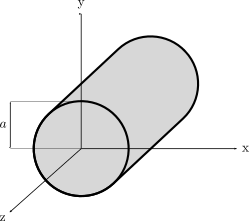
\includegraphics[scale = 1]{Figures/Apendice_A/apendiceA_3.pdf}
\caption{Condiciones de borde para una guía de onda cilíndrica.}
\label{fig_apA:3}
\end{figure}
%%%%
La componente del campo eléctrico tangencial a la pared metálica de la guía de onda se anula, por lo que:
%%%%
\begin{align}
&E_{\phi}\left(\rho = a\right) = 0\Longrightarrow\frac{\partial H_z}{\partial\rho}\left(\rho = a\right) = 0
\label{ec_apA:116}
\end{align}
%%%%
Aplicando las condiciones de borde \eqref{ec_apA:116}, se determina que:
%%%%
\begin{align}
&k_t = \frac{\chi '_{np}}{a}
\label{ec_apA:117}
\end{align}
%%%%
donde $\chi '_{np}$ son las raíces de las derivadas de las funciones de Bessel de primera especie, cuyos valores principales pueden obervarse en la tabla \ref{tabla_apA:1}
%%%%
\begin{table}[H]
\centering
\begin{tabular}{|c|c|c|c|c|c|c|}
\hline
\backslashbox{p}{n} & 0 & 1 & 2 & 3 & 4 & 5 \\
\hline
1 & 3,832 & 1,841 & 3,054 & 4,201 & 5,317 & 6,416\\
\hline
2 & 7,016 & 5,331 & 6,706 & 8,015 & 9,282 & 10,520\\
\hline
3 & 10,173 & 8,536 & 9,969 & 11,346 & 12,682 & 13,987\\
\hline
4 & 13,324 & 11,706 & 13,170 & 14,586 & 15,964 & 17,313\\
\hline
\end{tabular}
\caption{Raíces de las derivadas de las funciones de Bessel de primera especie.}
\label{tabla_apA:1}
\end{table}
%%%%
y las expresiones \eqref{grup_ec_apA:24} se reducen a:
%%%%
\begin{subequations}
\label{grup_ec_apA:25}
\begin{align}
\frac{\partial H_z}{\partial\rho} &= AC\cos\left(n\phi\right){J_n}'\!\left(\frac{\chi '_{np}}{a}\rho\right)
\label{ec_apA:118}\\
\frac{\partial H_z}{\partial\phi} &= - ACn\sen\left(n\phi\right)J_n\!\left(\frac{\chi '_{np}}{a}\rho\right)
\label{ec_apA:119}
\end{align}
\end{subequations}
%%%%
Las expresiones de los campos resultan:
%%%%
\begin{subequations}
\label{grup_ec_apA:26}
\begin{align}
E_{\rho} &= -j\frac{n\omega\mu K}{\rho\gamma_t^2}\sen\left(n\phi\right)J_n\!\left(\frac{\chi '_{np}}{a}\rho\right)
\label{ec_apA:120}\\
E_{\phi} &= -j\frac{\omega\mu K}{\gamma_t^2}\cos\left(n\phi\right){J_n}'\!\left(\frac{\chi '_{np}}{a}\rho\right)
\label{ec_apA:121}\\
E_z &= 0
\label{ec_apA:122}\\
H_{\rho} &= \frac{\gamma_zK}{\gamma_t^2}\cos\left(n\phi\right){J_n}'\!\left(\frac{\chi '_{np}}{a}\rho\right)
\label{ec_apA:123}\\
H_{\phi} &= -\frac{n\gamma_zK}{\rho\gamma_t^2}\sen\left(n\phi\right)J_n\!\left(\frac{\chi '_{np}}{a}\rho\right)
\label{ec_apA:124}\\
H_z &= K\cos\left(n\phi\right)J_n\!\left(\frac{\chi '_{np}}{a}\rho\right)
\label{ec_apA:125}
\end{align}
\end{subequations}
%%%%
donde $K = AC$ es una constante. Cada combinación de los índices $n$ y $p$ define un modo de propagación TE posible, que se designa como modo TE$_{\text{np}}$.

Empleando las expresiones \eqref{ec_apA:27} y \eqref{ec_apA:117}, la expresión resultante del factor de propagación $\gamma_z$ es:
%%%%
\begin{align}
&\gamma_z = \sqrt{k^2_t - k^2} = \sqrt{\left(\frac{\chi '_{np}}{a}\right)^2 - \left(\frac{2\pi f}{c}\right)^2}
\label{ec_apA:126}
\end{align}
%%
mientras que la frecuencia de corte se expresa como:
%%%%
\begin{align}
&f_c = \frac{c}{2\pi}\frac{\chi '_{np}}{a}
\label{ec_apA:127}
\end{align}
%%%%
Manipulando matemáticamente, las expresiones de $\beta$, $\lambda_g$ y $\eta_{TE}$ son las mismas que las halladas en la sección \ref{sec_apendice_a_guia_rect}: \eqref{ec_apA:65}, \eqref{ec_apA:66} y \eqref{ec_apA:67} respectivamente. La única diferencia es que hay que utilizar la expresión de la frecuencia de corte \eqref{ec_apA:127}.

Para el modo de propagación TE$_{11}$, las expresiones de las componentes de los campos resultan:
%%%%
\begin{subequations}
\label{grup_ec_apA:27}
\begin{align}
E_{\rho} &= - j\frac{\omega\mu K}{\rho\gamma_t^2}\sen\phi\,J_1\!\left(\frac{\chi '_{11}}{a}\rho\right)
\label{ec_apA:128}\\
E_{\phi} &= - j\frac{\omega\mu K}{\gamma_t^2}\cos\phi\,{J_1}'\!\left(\frac{\chi '_{11}}{a}\rho\right)
\label{ec_apA:129}\\
E_z &= 0
\label{ec_apA:130}\\
H_{\rho} &= \frac{\gamma_zK}{\gamma_t^2}\cos\phi\,{J_1}'\!\left(\frac{\chi '_{11}}{a}\rho\right)
\label{ec_apA:131}\\
H_{\phi} &= - \frac{\gamma_zK}{\rho\gamma_t^2}\sen\phi\,J_1\!\left(\frac{\chi '_{11}}{a}\rho\right)
\label{ec_apA:132}\\
H_z &= K\cos\phi\,J_1\!\left(\frac{\chi '_{11}}{a}\rho\right)
\label{ec_apA:133}
\end{align}
\end{subequations}
%%%%
y la frecuencia de corte:
%%%%
\begin{align}
&f_c = \frac{c}{2\pi}\frac{\chi '_{11}}{a}
\label{ec_apA:134}
\end{align}
%%%%
Si se considera una guía de onda cilíndrica con un extremo abierto, será el extremo abierto de la guía el que cumplirá la función de abertura. A los fines de resolver el problema de radiación, puede considerarse que los campos sobre la abertura son las componentes transversales de los campos en la guía de onda, por lo que:
%%%%
\begin{subequations}
\label{grup_ec_apA:28}
\begin{align}
\mathbf{E}_a &= - j\frac{\omega\mu K}{\rho\gamma_t^2}\sen\phi\,J_1\!\left(\frac{\chi '_{11}}{a}\rho\right)\!\versor{\uprho} - j\frac{\omega\mu K}{\gamma_t^2}\cos\phi\,{J_1}'\!\left(\frac{\chi '_{11}}{a}\rho\right)\!\versor{\upphi}
\label{ec_apA:135}\\
\mathbf{H}_a &= \frac{\gamma_zK}{\gamma_t^2}\cos\phi\,{J_1}'\!\left(\frac{\chi '_{11}}{a}\rho\right)\!\versor{\uprho} - \frac{\gamma_zK}{\rho\gamma_t^2}\sen\phi\,J_1\!\left(\frac{\chi '_{11}}{a}\rho\right)\!\versor{\upphi}
\label{ec_apA:136}
\end{align}
\end{subequations}
%%%%
Si las dimensiones de la abertura son grandes comparadas a la longitud de onda, los campos sobre la abertura $\mathbf{E}_a$ y $\mathbf{H}_a$ están relacionados entre sí a través de la expresión \eqref{ec_apA:77}; si además se toma:
%%%%
\begin{align}
&E_0 = - j\frac{\omega\mu K}{\gamma_t^2}
\label{ec_apA:137}
\end{align}
%%%%
las expresiones \eqref{grup_ec_apA:28} se reducen a:
%%%%
\begin{subequations}
\label{grup_ec_apA:29}
\begin{align}
\mathbf{E}_a &= E_{\rho}\,\versor{\uprho} + E_{\phi}\,\versor{\upphi} = E_0\,\dfrac{\sen\phi}{\rho}\,J_1\!\left(\dfrac{\chi '_{11}}{a}\rho\right)\!\versor{\uprho} + E_0\cos\phi\,{J_1}'\!\left(\dfrac{\chi '_{11}}{a}\rho\right)\!\versor{\upphi}
\label{ec_apA:138}\\
\mathbf{H}_a &= -\dfrac{E_{\phi}}{\eta}\,\versor{\uprho} + \dfrac{E_{\rho}}{\eta}\,\versor{\upphi} = - \dfrac{E_0}{\eta}\cos\phi\,{J_1}'\!\left(\dfrac{\chi '_{11}}{a}\rho\right)\!\versor{\uprho} + \dfrac{E_0}{\eta}\frac{\sen\phi}{\rho}\,J_1\!\left(\dfrac{\chi '_{11}}{a}\rho\right)\!\versor{\upphi}
\label{ec_apA:139}
\end{align}
\end{subequations}
%%%%